\documentclass[12pt]{report}
\usepackage[a4paper, margin=2cm]{geometry}
\usepackage[english]{babel}
\usepackage[figurename=Illustration]{caption}
\usepackage{tikz}
\usepackage{gensymb}
\usepackage{sidecap}
\usepackage{float}
\usepackage{hyperref}
\usepackage{makeidx}
\usepackage{titlepic}
\usepackage{mathtools}

\usepackage{xcolor}

\definecolor{papaya}{RGB}{255, 239, 213}

\usepackage{tcolorbox}

\newenvironment{note}{
\begin{tcolorbox}[boxrule=0pt]\textbf{Note}\newline
}{
\end{tcolorbox}
}

\newenvironment{warning}{
\begin{tcolorbox}[boxrule=0pt,colback=papaya]\textbf{Warning}\newline
}{
\end{tcolorbox}
}

\newcommand{\illustrate}[4][1]{
  \begin{figure}[H]
    \centering
    \includegraphics[width=#1\textwidth]{#2}
    \caption{#3}
    \label{#4}
  \end{figure}
}


\setlength{\parskip}{\baselineskip}
\setlength{\parindent}{0pt}
\makeindex

\title{
Rugged Frog's Polygon Pack
\newline
\textit{From Design to Construction}
}
\author{Arthur Van de Wiele}
\titlepic{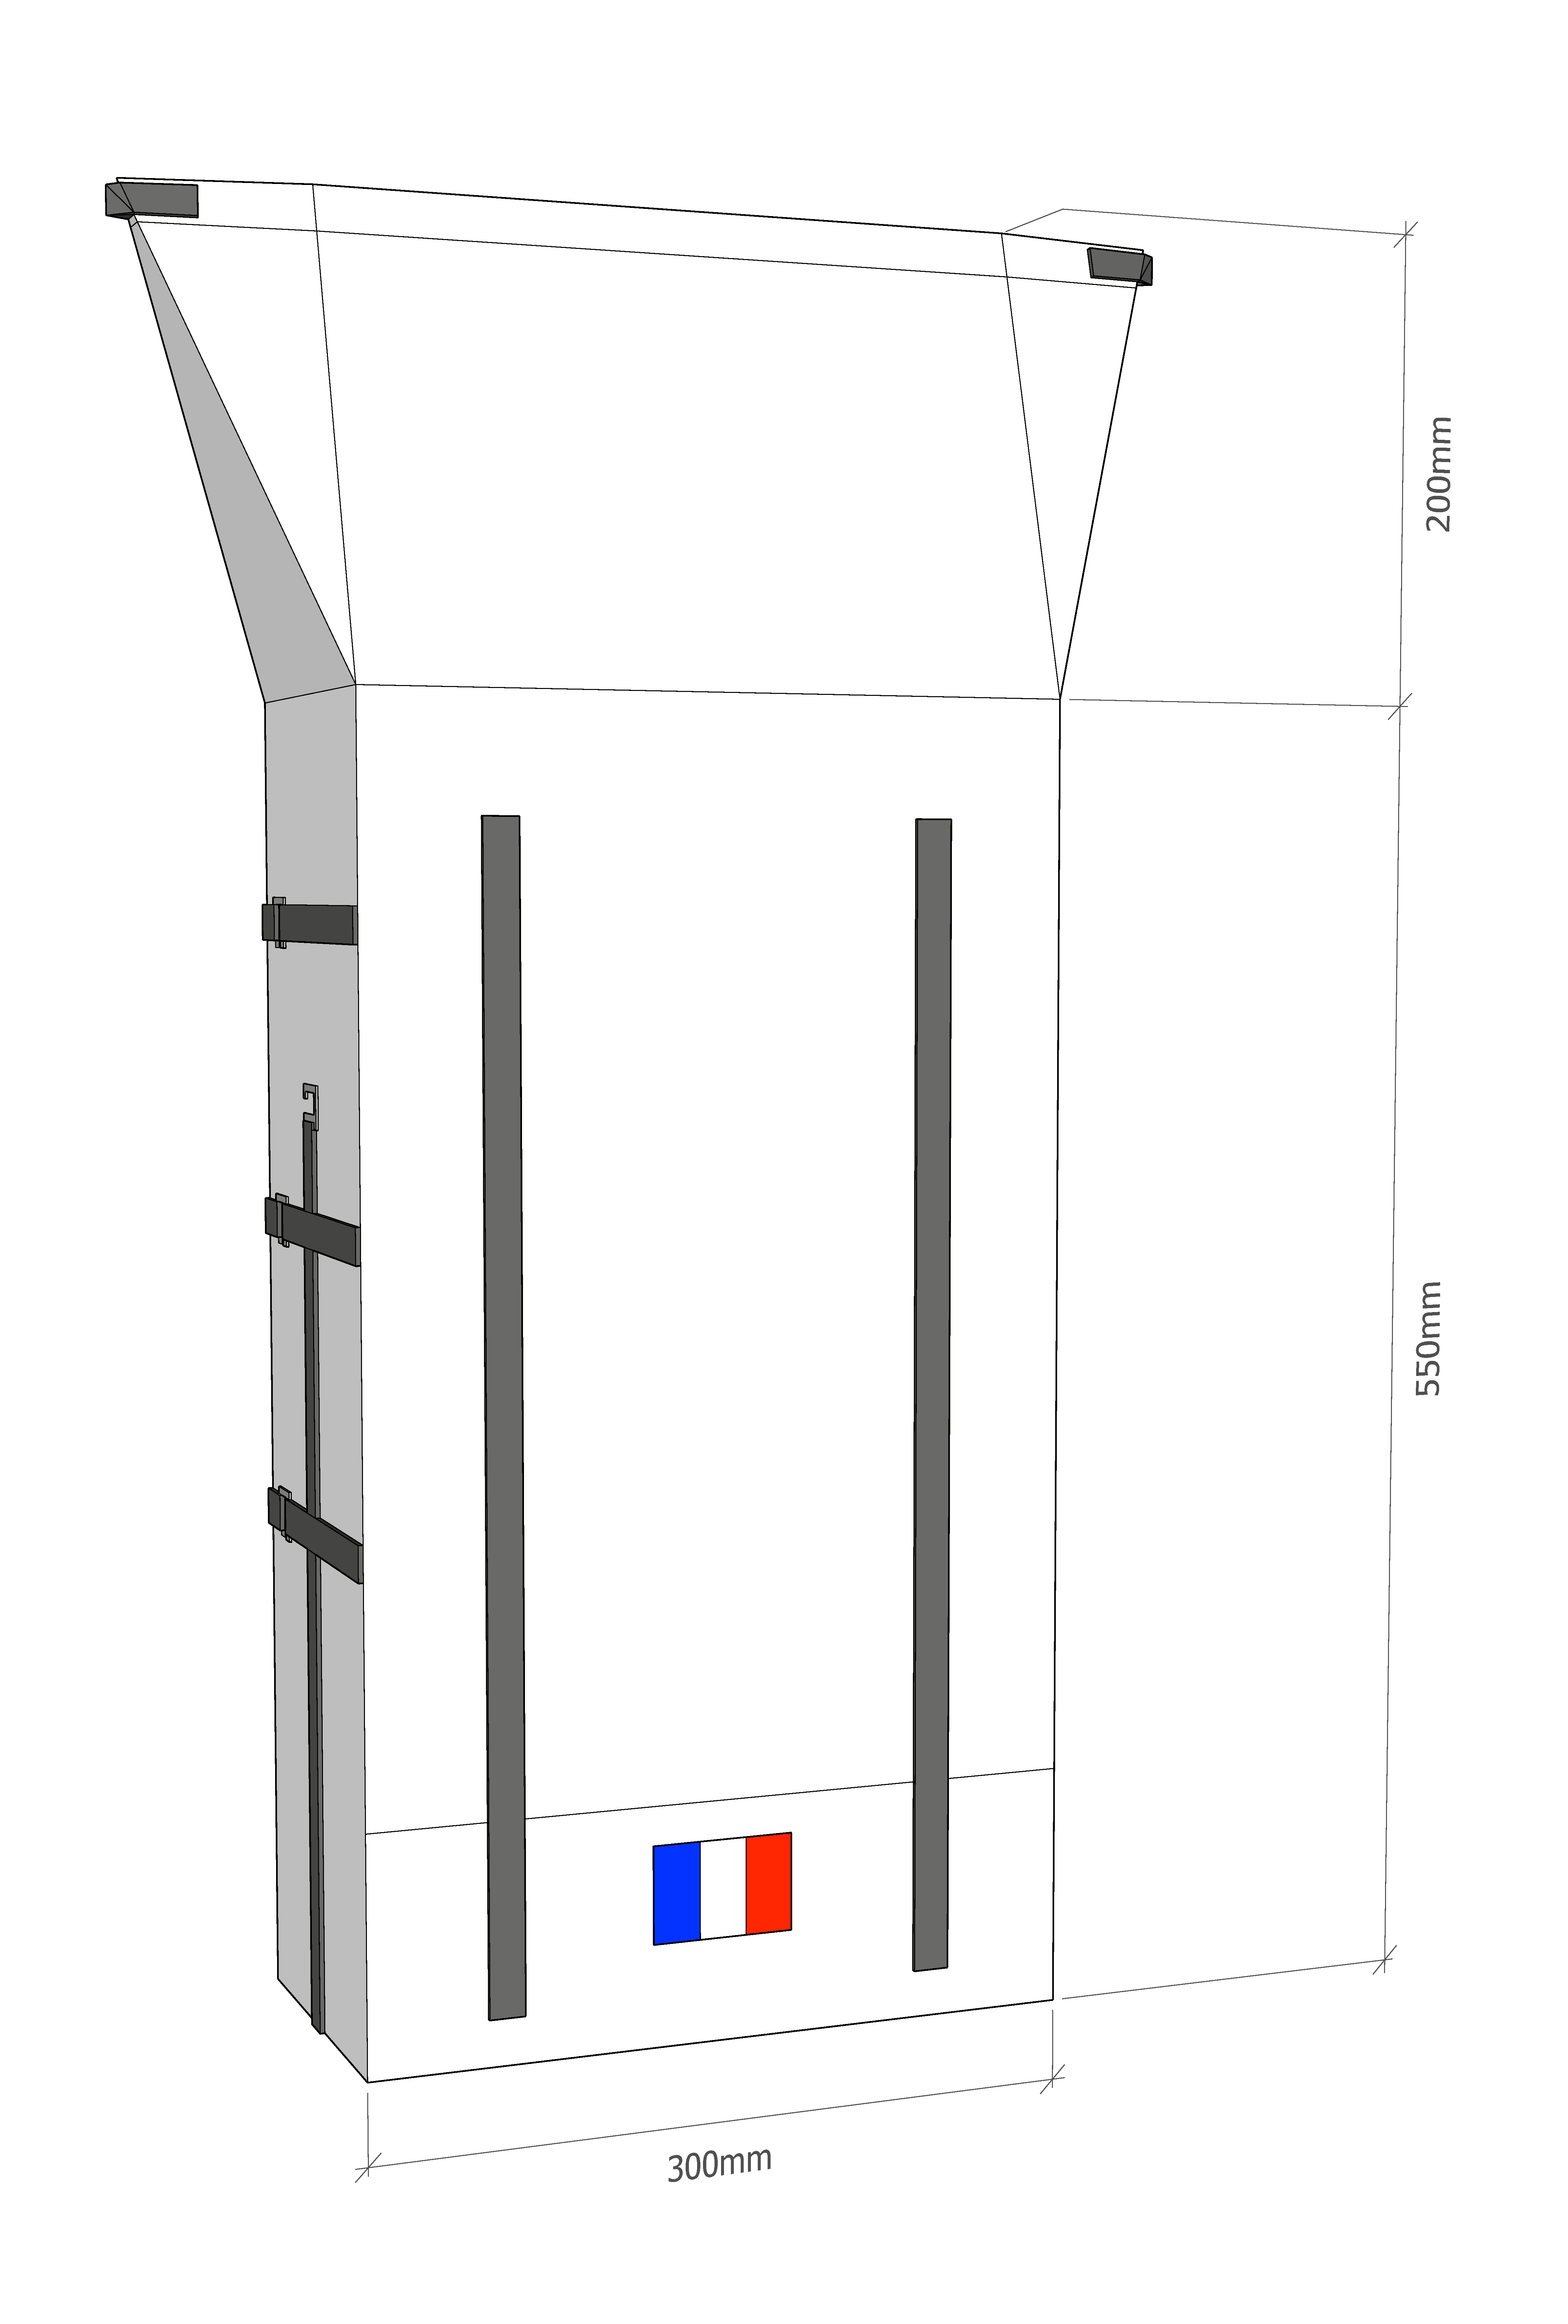
\includegraphics[width=.6\textwidth]{media/sketches/pack-full-3d-fr.pdf}}

\begin{document}
  \maketitle
  \tableofcontents

  \chapter{Introduction} \label{chap:intro}
First things first, when reading the following chapter, keep one thing in mind: I do my best to design lightweight backpacks, but I wouldn't push it so far as to calling them ultralight packs. There are highly specialised, very talented backpack makers out there who focus all their attention on ultralight hikers (and thru-hikers),  and they come up with amazing featherweight designs. Personally, I have a less drastic approach to weight loss in general, but I am still aiming at a substantial weight reduction without hampering the functionality of my packs.

\section{Foreword}
There is something about making my own outdoor gear that I can't get enough of. I have always been a maker to some extent, and - usually - my creations are very short lived. I've come to think of it as being more about the process, about the work I put into making something, and the learnings I get from it, rather than about the outcome itself.

For outdoor gear, it is still about the process, but the outcome is tangible to a much grater extent than anything else, as I can use it, abuse it, and improve upon every iteration. Take the example of backpacks: I can carefully plan every part of it, dedicate every feature to a particular problem I want to solve in a particular situation, and do tons of research, but then, I end up with something more than the sum of my work, something I'm going to enjoy (or hate) for miles to come, literally.


\section{How did it all start?}

The outdoors always helped me balance my somewhat stressful and chaotic work life with some blessed moments of calm and quiet. Before taking on sewing, I had spent a lot of time hiking around the world, and although I don't consider myself an ultralight backpacker, I do make conscious decisions on what to pack on a trip based on weight and versatility. At the end of the day, it always came down to my gear not being one hundred percent suited to my personal needs, and more often than not, ended up with me having to carry more than necessary.

Designing my own backpacks came quite naturally. I happened to own already a handful of packs already, each one with their pros and cons. I knew what I liked or disliked, what I used, and what I did not. I've always slightly modified my packs to remove unnecessary weight on them, just so I can focus on carrying the essential on a longer distance, or simply with less efforts. All that trimming brought up many questions - and answers - about the structure of today's backpack, their versatility, and by definition their average target group.

From there, the jump to making a complete pack was mostly about acquiring the skills, researching the fabrics and components, and gather tons of drawings. It's from those drawing that I stated putting together my first pack. Suffice to say, first attempts barely registered as functional, but I used the failures of each to improve the next pack, and the next, and the next. I started paying more and more attention to all the packs I can get my eyes and hands on, analysing more and more designs to build up some kind of a knowledge base on how others solved existing problems. On the other hand, I got started training, and kept on sewing together different kind of packs, using a multitude of fabrics building more and more complexity in each pack.


\section{A few words on backpacks in general}

\subsection{things one carries, and why it matters}

When you want to have a look at pack weight, you should first consider what exactly you are carrying. For a trip, the weight of my pack is divided in two categories:

\begin{itemize}
	\item My \textbf{base weight} is the weight of my gear, this account for my sleeping system, my clothing, my shelter, and - of course - the pack I carry everything in.
	\item Things like food, water, or the fuel for your stove, are weights which not only vary during a trip, but most importantly will differ from one trip to another. They are the \textbf{consumable} part of the weight you carry.
\end{itemize}

This separation in two categories finds its roots in a very simple truth: although you can be smart about what \textit{consumables} you carry, there is only so much weight you can avoid carrying  for your hydration and caloric needs (water can't be altered to weight less, and calories don't come from thin air). Base weight, on the other hand, can be tremendously altered by your choices of items, and how they function together as an ensemble.

If you are reading this, then you probably have done some research already on how to hike lighter, and by now you should be familiar with the big three things which everyone should pay attention to:

\begin{itemize}
	\item Sleeping system
	\item Shelter
	\item Backpack
\end{itemize}

They represent the most part of your base weight, and also are historically the most overlooked piece of equipment when it comes to shaving weight.

\subsection{Example of weight distribution}

If you want to design a backpack, you will need to understand how your gear consumes weight. It is crucial you understand the fine balance between weight and comfort. Every one is different, and will want different levels of comfort, but more so, every trip is different, and will require different pack construction. A simple example can be drawn from a commercial, highly comfortable trekking backpack, which is my go to for loads of 8-10kg, and a frameless, padless backpack I user for loads around 5kg.

This is taken from one of my trips and the following pie chart shows how weight distribution was with conventional gear. I put together this kit to wander the Annapurna Circuit Trek with a focus on \textit{warmth} and \textit{comfort} at high altitude. I had a lot of constrains with the weather as I was hiking for 3 weeks straight, with no expectation for being able to resupply anything other than consumables. In this part of the Himalayas, the altitude variations between 800m and 5400m means temperatures between +25\degree C to -30\degree C.

\input{media/graphics/base-weight-pie-anapurna}

As you can see in this example, the weight of my backpack at the time was competing with my -30\degree celsius down sleeping bag. And I can tell you, both the sleeping bag and the pack where too heavy for what I needed. Despite the fact that my pack was already touching the decently light category at 1.1kg for a very comfortable pack.

An example of shaving a lot of base weight happened in one of my last trip: a fast-paced hike of Scotland's Great Glen Way where I walked 130km in 4 days. For this trip, I had to carry a complete shelter and sleeping system, but not a lot of anything else. So I switched to a custom made ultralight backpack (around 350 grams) and some ultralight 1-person tent (630 grams) with a closed-cell foam sleeping pad (400g). I also used a down quilt instead of a sleeping bag (10\degree C comfort, 395 grams) which was definitely too light.

In should become obvious weight if often a tradeoff with comfort. In that regard, every being different, you will have to find your "sweet spot" on your own.

\input{media/tables/baseweight-comparison-annapurna-scotland}

\subsection{Weight categories \& purpose}

The purpose of a pack is obviously to carry things. But the way I will use it make a huge difference in the way I design a pack. For example, I care little for inside pockets, I always carry some stuff outside my pack, I usually lug around loads between 3 to 8 kilograms (depending on how long I'm hiking for, and in which conditions) but most of my gear compresses well, so 40 litres is usually good enough.
For loads equivalent to 40 litres weighing 7 to 9kilograms, most commercially available backpacks oscillate between 1.20 and 1.80 kilograms, and specialised ultralight backpacks can go down to 300 grams.



\chapter{My teeny tiny workspace} \label{chap:workspace}
If there is one thing that is important to any kind of creative process, it is space. I just wanted to document my project table, to show you that the bare essentials you need are not that many. Sure, having a better working space - bigger, better organised, with more stuff - would be nice, but I have all I need right here.

\section{Different needs, different spaces}
For those who know me, the least one can say is that I like order. And trust me, a workshop can get messy ! I usually fold fabrics, and sort components, in a well organised system, stored away in different boxes when I’m not sewing anything. That way, I can fetch exactly what I need (or I think I need) when I need it. I simply have a much better space to just let the ideas flow when my table is not drowning under cuts of different material, with sewing thread everywhere, components lying around on the table and on the floor... Well, you get the picture.

Most of the time I spend at my workspace is divided in three phases.

\begin{itemize}

  \item Research and drawing
  \item Quick prototyping and trying things out
  \item Putting together a complete pack

\end{itemize}

For each of this phases, I re-arrange my workspace a little bit different. They are, at the end of the day, the same place, but maybe I can give you a few pointers as to where to start. The rest will be up to you.

\illustrate{media/images/workspace-1}
{My workspace when I cleaned it up}
{img:workspace-1}


\section{Research and drawing space}
I find most of my inspiration on the web. There are people out there who have better ideas than mine, and I don’t shy away from blatantly experimenting, learning and copying any concept or design I like. I am dedicating the entire chapter \ref{chap:inspiration} to how and where I find inspiration, so let’s just boil it down to the essentials here and look at the image \ref{img:workspace-2}.

\begin{figure}
  \includegraphics[width=\textwidth]{media/images/workspace-2}
  \caption{My desk for researching and drawing new packs}
  \label{img:workspace-2}
\end{figure}

\begin{description}

  \item[Paper] I prefer a plain white fine grain A3 Canson sketchbook (I just love the space and the grain, and the lack of constrains of plain paper) but any paper/sketchbook would do of course. I stay away from millimetre paper because I don’t need accurate drawings.

  \item [Ball Pen] Just trust me, and don’t use a pencil and an eraser. It’s way better to draw, make mistakes, and draw again and again. Keep your complete history of designs. Take notes on them regarding why you would have erased it, what you think works and doesn’t.

  \item [Cutting Mat] A cutting mat is awesome to keep around as it gives a scale to anything you find online.

  \item [Measuring Tape] A tailor’s tape measure, so I can grab any of my packs and take a fresh set of measures to scribble it into a drawing. Any ruler would do, but working with fabrics and a rigid ruler is not ideal.

  \item [References] I keep some kind of inventory of the components I’ve tried and liked. I have tried loads of different webbing types and sizes, different buckles, different clips. Keeping track of whether they work together or not is essential. This is great to already get an idea of how I can put something together. See section \ref{sec:gear-database} for more details.

\end{description}


\section{Sewing workspace}
If there is one thing that took me a while to get a hang of, is how to organise myself when working with meters of fabric, a ton of stuff lying on the desk, and a sewing machine standing in my way most of the time.



\chapter{Find the inspiration} \label{chap:inspiration}
\section{The manufacturers I keep an eye on}
There are too many manufacturers of backpacks for me to keep looking at everyone one of them. But over time, and in the lightweight to ultra-lightweight community, there are a couple of well respected names I always look forward to dissecting and use for reference. Smaller names tend to innovate more, where better established brands have more diversity and complexity. Both are a fantastic source for inspiration.

Generally speaking, UL packs have a lot in common, so I don’t focus all my attention on ultralight gear maker, instead, I do all I can to find innovative ways of dialling down on pack weight without compromising comfort too much.

Here is a very short list of where I look for inspiration every once in a while:

\begin{description}

  \index{reddit}
  \item [Reddit] Oh yeah, that’s where you want to go to get in touch with the community of fantastic trekker/hikers who make packs. There are plenty of platform and communities out there, I personally roam these the most: \textit{r/ultralight} and \textit{r/myog}.

  \item [HMG] Hyperlight Mountain Gear is well respected business for a variety of ultralight gear, and I just love their pack designs. I unfortunately do not own one (yet) as I find them a little pricey. But who knows.

  \item [KS (Kinpu San)] ultralight gear is a fantastic one-man custom pack making business held by Laurent, out of Japan. I personally own his Tao pack, and I’ve had very comfy, very long days of hiking with it. This was the pack I brought with me to a short trek in Scotland, and the simple features held great in all weather with a light load (6-7kg).

  \item [Osprey] Over the years, Osprey has made a name for themselves by making very decently priced, sturdy and not too heavy packs. I’ve own an Exos for a few years, and still take it for a spin every once in a while. This was the pack I brought with me in the Himalayas, and I couldn’t have been happier with its performance with a medium load (9kg).
  \item [Sierra Design] A very interesting brand if only for the fact that they don’t do 100\% symmet- rical packs ! Think about how often you strap the same thing on the same side of the pack ? Well, maybe having a symmetrical design is not the best option. I certainly like the concept.

  \item [ÜLA] ÜLA is definitely a good place to look at. It’s a refreshing combination of ultralight - very simple - designs, with a more complex cut (not the usual rectangle pack) then most.

  \item [MLD] Mountain Laurel Design is also one of my personal favourite, although I never had a chance to try one out. They work from basic shapes, but have tons a very smart details that make it a great selection of packs.

  \item [ZPacks] Their packs are simple but effective. And they have a frame ! Which is quite rare for UL designs. I haven’t had a chance to wear one yet and see how it carries.

  \item [Decathlon] A big outdoor name from France who does more research on fabrics and designs than people might think. They do lack specialised equipment, but instead try to innovate a lot, so I always keep an eye on what they come up with. I’ve own many of their day packs, and have gotten my hand on many different trekking/hiking designs, and they all came up surprisingly close to what I consider lightweight.

\end{description}


\section{Learnings}
\subsection{Database}\label{sec:gear-database}

\begin{figure}[H]
  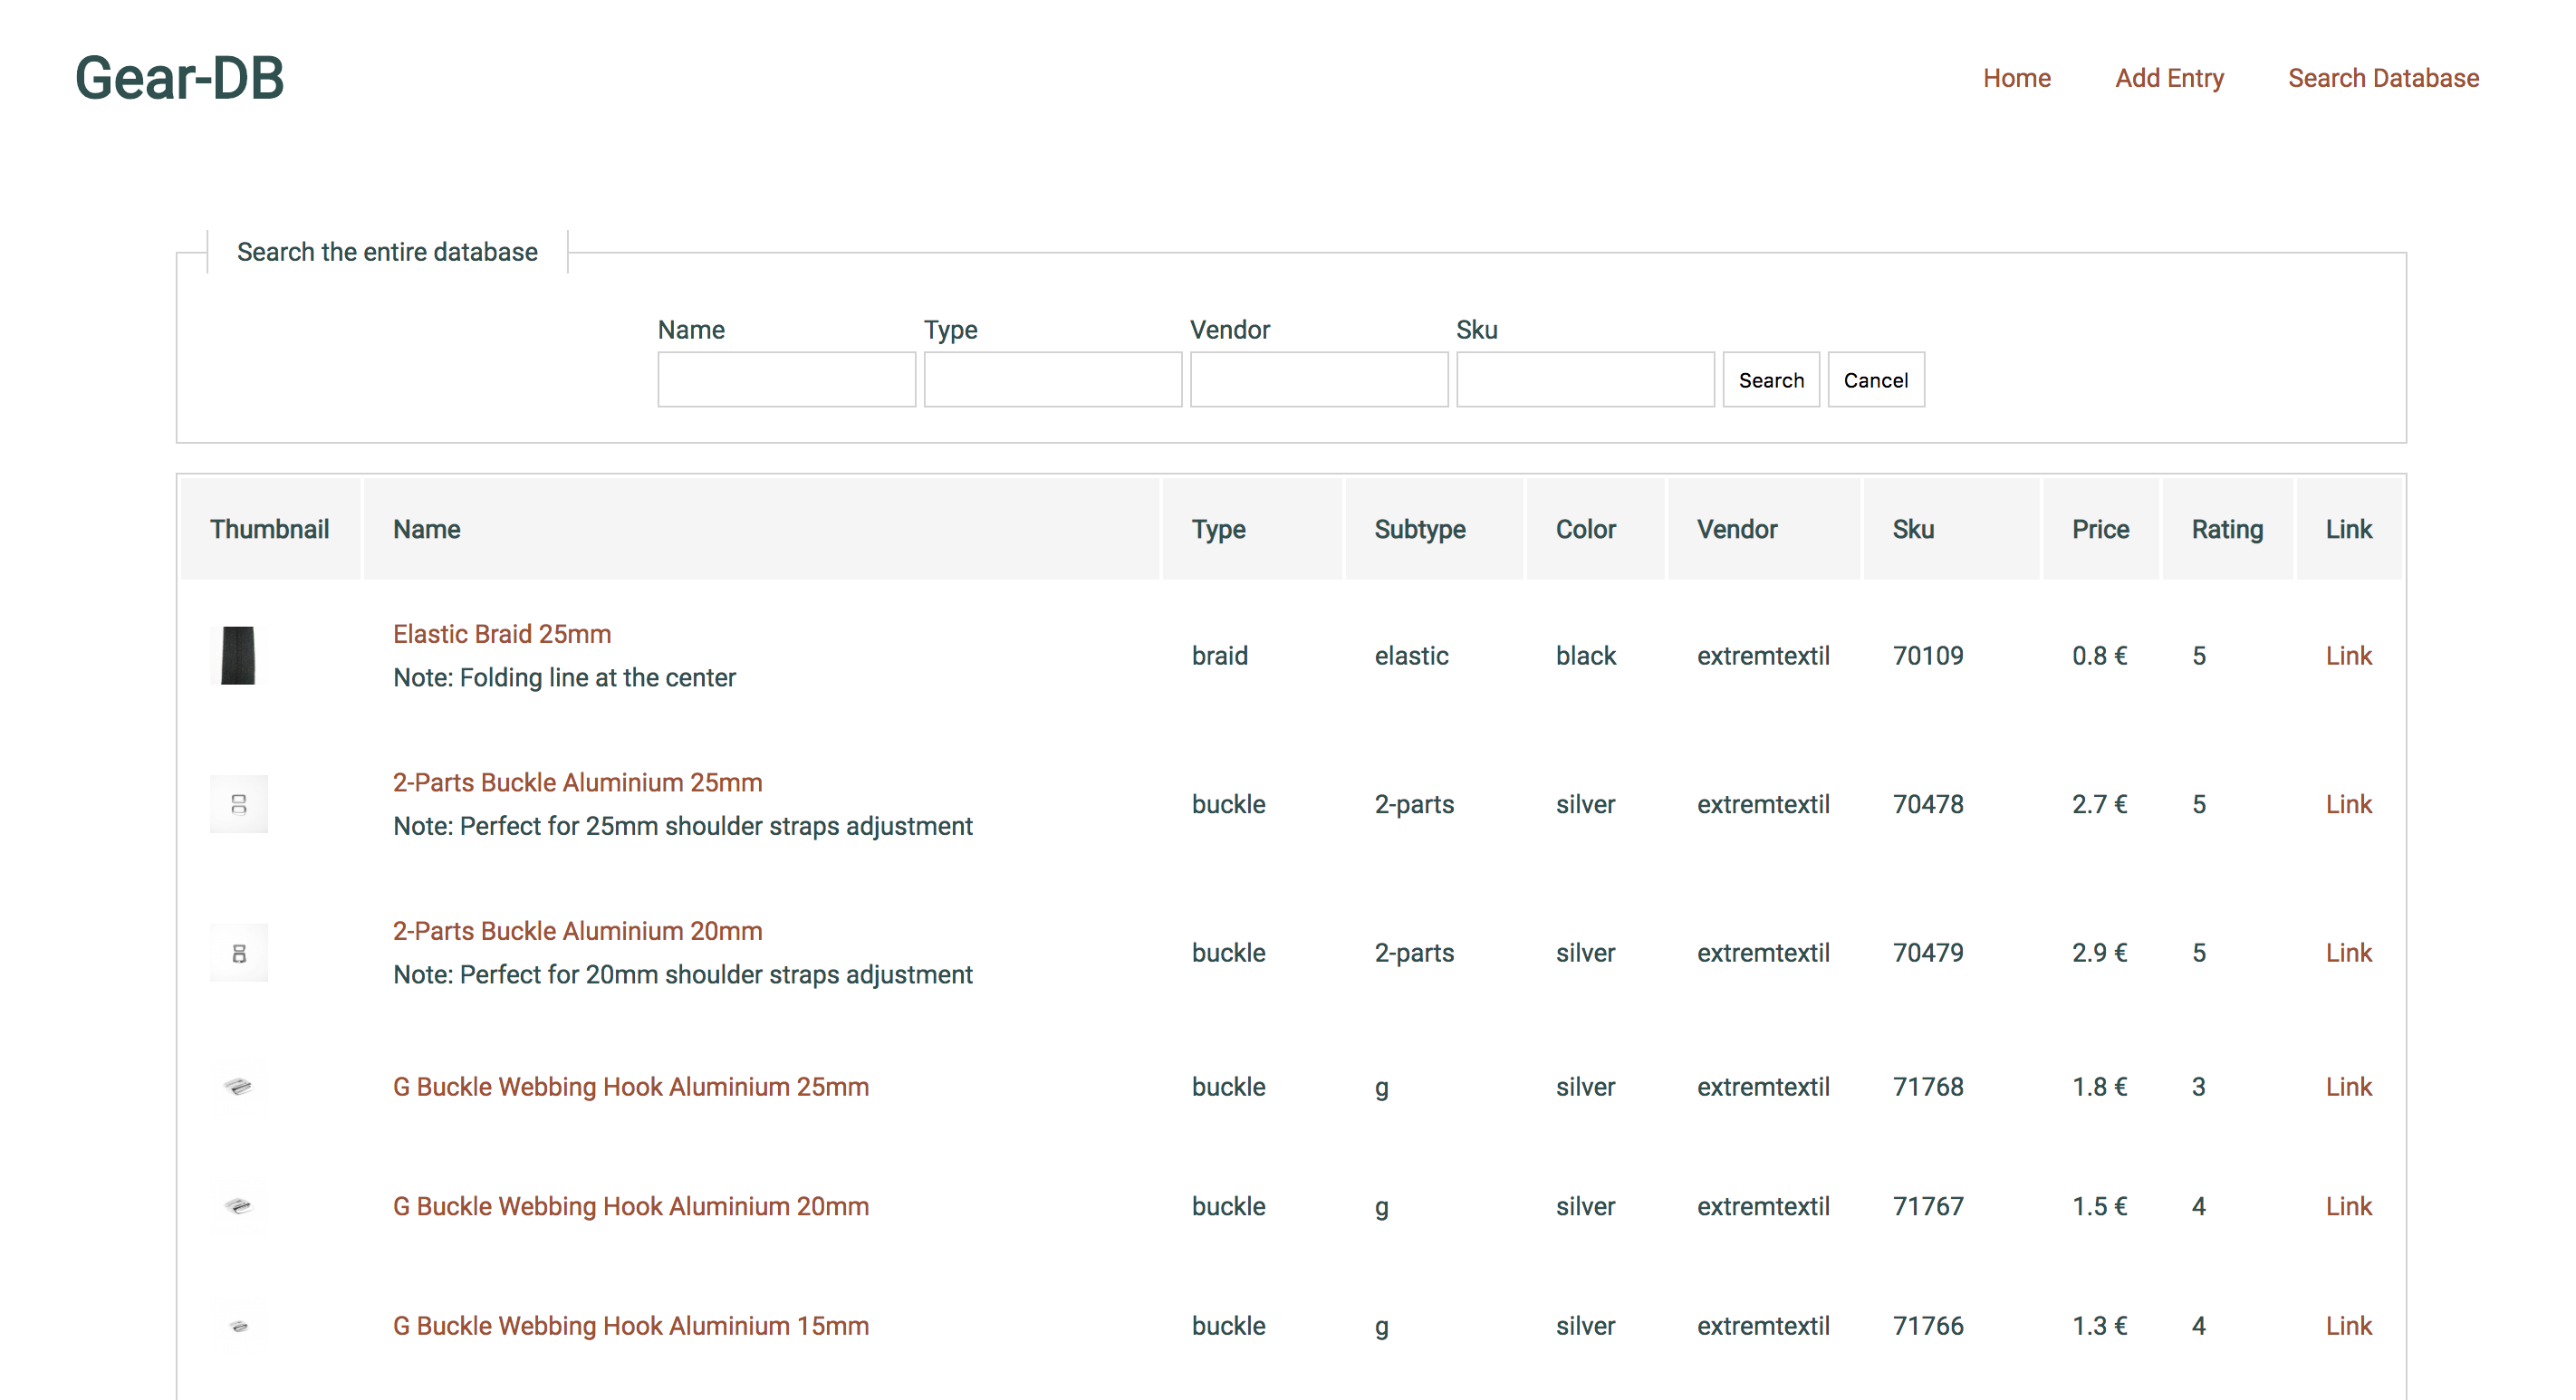
\includegraphics[width=\textwidth]{media/images/gear-database}
  \caption{Extract of the gear database}
\end{figure}



\chapter{Drawing up a concept} \label{chap:drawing}
\section{Strip it down to essentials}
There is a backpack for any situation, and it's always interesting to look at what others are doing. I have a few backpacks - both commercial and custom made - at home I can analyse inside and out to figure out what I'm interested in. And there is a plethora of detailed pictures and designs on the web, ranging from home made MYOG articles, to high-end ultralight gear manufacturer, to cost-effective mass production design.


\section{Features}
When I try to define a set of features for a new backpack, the first step is to define the style and application of my design:

\begin{description}

  \item [Aesthetics] As basic as this sounds, I always enjoy a pack that doesn't look like I put it together in a few minutes. This will cost some extra fabric and or components in most cases, but I prefer it that way.

  \item [Load] The padding, weight balance and distribution, boiling down to the basic shape of a backpack is driven by how much weight it will need to carry. This impacts the construction of the shoulder straps, and the of the hip belt as well.

  \item [Weight] The basic weight of the backpack is tied to its construction, the materials used and its shape, the features I build in, etc... I rarely use this as a target, rather, I review everything else and try hard not to over-engineer a pack to limit the extra weight.

  \item [Attachments] There is a ton of options to attach things to a backpack. In outdoor cases, I often have a tent and/or sleeping pad attached on the sides and bottom of the pack, I also use walking poles which I often strap on the side of the pack.

  \item [Pockets] Whether inside or outside, pockets are an essential part of a pack. Depending on how you usually organise your pack, you would consider internal compartments, inside pockets, outside mesh pockets, and so on. I personally don't care much for pockets, as I organise my gear in stuff sacks. But I often need to attach/store things on the outside for easy access, or for drying.

  \item [Closure] There is a ton of different way to close a backpack. To name but a few, I often consider roll tops, zippers, velcro, tie-ins or a mix of these.

  \item [Padding] Padding can be essential, or completely superfluous depending on what you carry, and how you carry it. I always build in a sleeve of some kind following the entire width and length of the pack to be able to add/remove foam padding depending on the trip.

  \item [Hip-Belt] For me, and essential part of any hiking/trekking pack. The rare packs I built without a hip-belt, I gave away because I never use them. Now whether I want the hip-belt complete with padding, or just a simple strap depends on the weight I plan on carrying. But it's always a good weight investment.

\end{description}


\section{Drawings}

\section{Measurements}

\section{Mock-Ups}


\chapter{Fabrics and Materials} \label{chap:materials}
\section{What to look for in a fabric}
I have spent quite a few bucks on different kinds of fabrics. There has been a few which really stood out from the rest by how strong they feel, or how easy they are to work with. There is a few things I'm looking for in the fabrics I use apart from the aesthetics:

\begin{description}

  \index{ripstop}
  \item [Ripstop] A backpack will get punctured, scratched, tossed around, overloaded and so on. If there is one thing I expect from the fabric, is that it survives for the duration of my trip no matter what tear and wear the pack goes through. Ripstop treatment is the process of interweaving a stronger filament at short intervals within the fabric, with a recurring pattern - say 5 mm by 5 mm squares - so that a tear in the fabric will be stopped by the stronger thread. It also helps the sewing process by offering anchors, and makes a fabric overall much more durable.

  \index{coating}
  \index{waterproof}
  \item [Water resistant coating] There is one thing that does not work well for traveling light, and it's having a fabric that absorbs water, making the pack much heavier than it should be. There is plenty of methods for coating a fabric, and there is enough demand for waterproof fabrics that the price of coated versus uncoated is close enough not to even care.

  \index{humidity}
  \item [Soaking resistance] Different fabrics come with different blends of material. Some of these materials' fibres resist much better to water than others. When I am considering a fabric, the water resistant coating is one thing, but it's ability to not get heavier with rain or humidity is almost as important. As the fabric does not weight more, and does not need drying.

\end{description}


\subsection{Order samples first}
Any self-respecting fabrics retailer will offer sample sets. Use them! I cannot stress that enough ! There no amount of research in the world that will give you a feel for a fabric. But a few bucks spent on acquiring a complete set of samples for what you need will. Have a look at the illustration \ref{img:fabrics-sample-set} to know what I mean by that.

\begin{figure}[H]
  \includegraphics[width=\textwidth]{media/images/fabrics-sample-sets}
  \caption{My beloved sample box}
  \label{img:fabrics-sample-sets}
\end{figure}


\section{My choice for fabrics}

\subsection{Heavy Duty Cordura}
\index{cordura}
Cordura is a fantastic fabrics to work with, especially coated. Uncoated, it's a rather soft fabric (depending on the denier it comes in) and frays very easily. One thing you should consider is that coated Cordura is much stiffer than uncoated, resulting in you probably needing a lower denier then uncoated. Denier is the rating of the thread of fibre used to weave the fabric, the higher the denier, the heavier and more durable the fabric.

\index{nylon}
As it is mostly comprised of nylon fibres (normally solely, but it sometimes comes with a cotton blend), it does not soak up water or moisture much, meaning its weight when wet is not significantly higher than when dry.

Cordura is a great fabric for parts of a backpack which will have to endure more abrasion and stress than the rest. This is usually true of the bottom part of a pack, when it is standing on the ground, and when items inside apply pressure at certain points.

\index{cordura}
\begin{figure}[H]
  \includegraphics[width=\textwidth]{media/images/fabrics-cordura-set-1}
  \caption{Cordura sample set}
  \label{img:fabrics-cordura-set-1}
\end{figure}

\index{cordura}
\begin{figure}[H]
  \includegraphics[width=\textwidth]{media/images/fabrics-cordura-set-2}
  \caption{Close-up of different denier Cordura weaves}
  \label{img:fabrics-cordura-set-2}
\end{figure}


\subsection{Lightweight Ripstop Synthetic Fibres}
\illustrate{media/images/fabrics-coated-set}
{Example of coated fabrics}
{img:fabrics-coated-set}

\illustrate{media/images/fabrics-tent-set}
{Example of lightweight tent fabrics (mostly Nylon)}
{img:fabrics-tent-set}


\subsection{Padding with 3D Mesh}
\illustrate{media/images/fabrics-3d-mesh-set}
{Example of 3D mesh}
{img:fabrics-3d-mesh-set}


\subsection{Padding with closed-cell foam}

\subsection{Multipurpose Mesh}
\illustrate{media/images/fabrics-mesh-set}
{Example of Multipurpose Mesh and Netting}
{img:fabrics-mesh-set}


\section{Tried and True Components}
\illustrate{media/images/components-1}
{Commonly used components}
{img:components-1}

\illustrate{media/images/components-2}
{Commonly used components}
{img:components-2}

\illustrate{media/images/components-3}
{Commonly used components}
{img:components-3}




  \cleardoublepage
  \phantomsection
  \addcontentsline{toc}{chapter}{\listfigurename}
  \listoffigures

  \cleardoublepage
  \phantomsection
  \addcontentsline{toc}{chapter}{\listtablename}
  \listoftables

  \cleardoublepage
  \phantomsection
  \addcontentsline{toc}{chapter}{\indexname}
  \printindex

\end{document}
